\documentclass{article}
\usepackage{graphicx} % Required for inserting images
\usepackage{gensymb,amsmath,amsfonts,amssymb,float,enumerate}
\usepackage{multicol,bm,subcaption}
\usepackage{subdepth}
\usepackage{multirow}
\usepackage{makecell}
\usepackage{hyperref}
\usepackage{xcolor}
\usepackage{soul}
% \usepackage{algorithm}
% \usepackage{algpseudocode}
% \usepackage[ruled,noline,noend]{algorithm2e}
% \usepackage{csquotes}

\title{The History Behind Leap Year}
\author{
    Nawriz Ahmed Turjo (2105032)
}
\date{\today}

\begin{document}

\maketitle

\section{Introduction}
% $a_0^1$
A leap year is a calendar year that contains an additional day compared to a
common year \cite{meeus1991}. This article covers the development of the leap year system and
its importance in keeping our calendar aligned with Earth’s revolution around
the sun.
\section{History}
\textbf{\textcolor{blue}{Did you know?}} The Earth takes about 365 days to orbit the Sun, but it’s not
exactly 365. In fact, it’s around  \textcolor{red}{\st{365}} \textcolor{green}{365.24} days.
\subsection{Julian Calendar}
Introduced by Julius Caesar (Figure \ref{fig:julius}) in 45 BC, the``Julian Calendar'' included
a leap year every four years. This was necessary because the solar year
is approximately 365.25 days long.
\subsection{Gregorian Calendar}
The modern leap year system was developed under Gregory XIII (Figure \ref{fig:gregory}) in
1582. In the ``Gregorian Calendar", leap years are introduced every four years,
except years divisible by 100 but not divisible by 400.
\section{Leap Year Rules}
The rules for calculating a leap year can be summarized as:
\begin{enumerate}
    \item \textbf{A year is a leap year if:}
    \begin{enumerate}
        \item It is divisible by 4 and not divisible by 100, or
        \item It is divisible by 400.
    \end{enumerate}
    \item \textbf{A year is \textit{NOT} a leap year \underline{in all other cases}.}
\end{enumerate}
\begin{figure}[ht]
    \centering
    \begin{subfigure}[b]{0.45\textwidth}
        % \raggedleft
        \hfill
        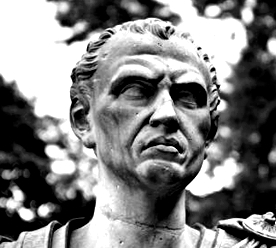
\includegraphics[width=0.8\textwidth]{julius.jpg}
        \caption{Julius}
        \label{fig:julius}
    \end{subfigure}
    \begin{subfigure}[b]{0.45\textwidth}
        % \raggedright
        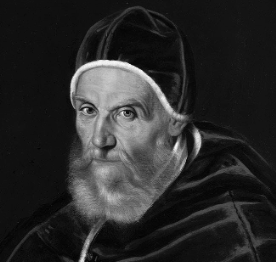
\includegraphics[width=0.75\textwidth]{gregory.PNG}
        \caption{Gregory}
        \label{fig:gregory}
    \end{subfigure}
    \caption{Pioneers of Modern Calendars}
    \label{fig:historical_figures}
\end{figure}

\section{Leap Year Calculation Formula}
The formula to determine if a year \textit{Y} is a leap year (or not) is written below.
\begin{equation}
    \mathrm{Leap\ Year} = 
    \begin{cases}
        \textbf{True}, & \text{if } (Y \% 4 = 0 \ \&\& \ Y \% 100 \neq 0) \ \| \ Y \% 400 = 0 \\ \nonumber
        \textbf{False}, & \text{otherwise}
    \end{cases}
\end{equation}
\\
Some examples of leap year calculations are shown in Table~\ref{tab:my-table}.

% Please add the following required packages to your document preamble:
% \usepackage{multirow}
\begin{table}[ht]
\centering
\begin{tabular}{|c|ccc|c|}
\hline
\multirow{2}{*}{\textbf{Year}} & \multicolumn{3}{c|}{\textbf{Divisible By}}                                            & \multirow{2}{*}{\textbf{Leap Year?}} \\ \cline{2-4}
                               & \multicolumn{1}{c|}{\textbf{4?}} & \multicolumn{1}{c|}{\textbf{100?}} & \textbf{400?} &                                      \\ \hline
1900                           & \multicolumn{1}{c|}{Yes}         & \multicolumn{1}{c|}{Yes}           & No            & No                                   \\ \hline
2000                           & \multicolumn{1}{c|}{Yes}         & \multicolumn{1}{c|}{Yes}           & Yes           & Yes                                  \\ \hline
2024                           & \multicolumn{1}{c|}{Yes}         & \multicolumn{1}{c|}{No}            & No            & Yes                                  \\ \hline
\end{tabular}
\caption{Leap Year Calculation Examples}
\label{tab:my-table}
\end{table}


\section{Importance}
The Earth takes approximately 365.24 days to complete one orbit around the sun. This discrepancy accumulates, and leap years help correct it. Without leap years, seasons would gradually drift over time.

\section*{Disclaimer}
The article is designed with the sole purpose of evaluating students' \LaTeX\ proficiency.

\bibliographystyle{plain}
\bibliography{ref}
\end{document}
